% Copyright 2026 Sreeram Anil
% SPDX-License-Identifier: CC-BY-4.0
% =============================================================================
%  Iterated extended Kalman filter — classical Kalman family
% =============================================================================
\chapter{Iterated Extended Kalman Filter (IEKF)}
\label{ch:iekf}

\section*{At a glance}
\begin{tabular}{@{}l>{\raggedright\arraybackslash}p{0.76\textwidth}@{}}
Family & classical Kalman \\
Header & \texttt{include/estkit/filters/iekf.hpp} \\
Registered name & \texttt{IEKF} \\
State dimension & $n_x = 4$ (cell model) --- generic in $n_x, n_u, n_y$ \\
Cost per step & $\mathcal{O}(J n_x^3)$, $J\le5$ iterations; $0.56$--$0.60\,\SI{}{\micro\second}$/step \\
Primary references & \cite{jazwinski1970,bellcathey1993,gelb1974} \\
\end{tabular}

\section{Motivation and aerospace/BMS relevance}
The EKF linearises the measurement function at the \emph{prior} mean $\xminus$. That is the
only point available before the measurement arrives, but it is the wrong point: after the
update the state is somewhere else, and if the innovation is large the Jacobian used to
compute the gain describes the wrong part of the nonlinearity. The classical cure, already in
Jazwinski's 1970 book~\cite[\S8.3]{jazwinski1970}, is to iterate --- relinearise at the
updated estimate and repeat the update until it stops moving.

Bell and Cathey~\cite{bellcathey1993} identified the recursion as Gauss--Newton applied to
the maximum-a-posteriori cost, which turned a heuristic into an optimisation algorithm with
known convergence behaviour and made it clear what the filter is actually computing: the
posterior \emph{mode} rather than a one-step linear approximation of the mean.

In BMS terms the relevant situation is a large voltage innovation: first power-up with an
unknown SOC, recovery after a sensor dropout, or a step change in load that the model gets
wrong. The OCV curve of an NMC/graphite cell is markedly nonlinear near the ends of the SOC
window, so a $0.3$\,V innovation corresponds to very different SOC corrections depending on
where the tangent is taken. In GNC the same argument is made for angles-only navigation and
for terrain-relative navigation, where a single measurement can carry a large correction.

\section{Problem statement and assumptions}
Model \eqref{eq:ekf-proc}--\eqref{eq:ekf-meas}. The time update is the EKF's. For the
measurement update, given the prior $\xminus_k$, $\Pminus_k$ and the observation $\vy_k$,
consider the maximum-a-posteriori (MAP) problem
\begin{equation}
\xplus_k = \argmin_{\vx}\; J(\vx), \qquad
J(\vx) = \tfrac12\norm{\vx - \xminus_k}^2_{(\Pminus_k)\inv} + \tfrac12\norm{\vy_k - h(\vx,\vu_k)}^2_{\mR\inv},
\label{eq:iekf-map}
\end{equation}
where $\norm{\bm{a}}^2_{\bm{M}} := \bm{a}^\T\bm{M}\bm{a}$. If $h$ were affine, $J$ would be a
quadratic whose minimiser is the EKF update; in general \eqref{eq:iekf-map} must be solved
iteratively. The assumption is that $h$ is twice differentiable and that $J$ has a unique
local minimum in the region of interest.

\section{Derivation}
Apply Gauss--Newton to \eqref{eq:iekf-map}. Writing $\mH_j = \partial h/\partial\vx|_{\vx_j}$
and linearising the residual $\vy_k - h(\vx,\vu_k)$ about the current iterate $\vx_j$,
\begin{equation}
J(\vx) \approx \tfrac12\norm{\vx-\xminus_k}^2_{(\Pminus_k)\inv}
 + \tfrac12\norm{\vy_k - h(\vx_j,\vu_k) - \mH_j(\vx-\vx_j)}^2_{\mR\inv}.
\label{eq:iekf-quad}
\end{equation}
Setting the gradient of \eqref{eq:iekf-quad} to zero and using the matrix inversion lemma to
turn the information-form solution into a gain form gives the iteration
\begin{align}
\mK_j &= \Pminus_k\mH_j^\T\left(\mH_j\Pminus_k\mH_j^\T + \mR\right)\inv, \label{eq:iekf-K}\\
\vx_{j+1} &= \xminus_k + \mK_j\left[\vy_k - h(\vx_j,\vu_k) - \mH_j\left(\xminus_k - \vx_j\right)\right],
\qquad \vx_0 = \xminus_k. \label{eq:iekf-iter}
\end{align}
The bracketed quantity is the residual that the linearised measurement predicts \emph{at the
prior mean}: for $j=0$ it reduces to the ordinary innovation $\vy_k - h(\xminus_k,\vu_k)$, so
\textbf{one iteration reproduces the EKF exactly}. The correction term
$-\mH_j(\xminus_k - \vx_j)$ is what keeps the prior anchored at $\xminus_k$ while the
expansion point moves.

Bell and Cathey~\cite{bellcathey1993} show that \eqref{eq:iekf-iter} is precisely the
Gauss--Newton step for \eqref{eq:iekf-map} with the Gauss--Newton Hessian approximation
$\nabla^2 J \approx (\Pminus_k)\inv + \mH^\T\mR\inv\mH$, hence: (i) it converges locally at a
rate governed by the residual size times the curvature (quadratic for zero-residual
problems), (ii) it may diverge for large residuals, which is why a damping factor
$\theta\in(0,1]$, $\vx_{j+1} = \vx_j + \theta\,\Delta_j$, is retained as an option, and
(iii) the natural covariance is the inverse Gauss--Newton Hessian evaluated at the solution,
\begin{equation}
\Pplus_k = \left[(\Pminus_k)\inv + \mH_J^\T\mR\inv\mH_J\right]\inv
 = (\mI - \mK_J\mH_J)\Pminus_k,
\label{eq:iekf-cov}
\end{equation}
implemented in Joseph form. The implementation uses the $(\mH_J,\mK_J)$ of the last executed
step, which makes the $J=1$ case bit-identical to the EKF (verified: max
$\abs{\Delta\vx}=0$, max $\abs{\Delta\mP}=0$ over a full mission) and is immaterial at
convergence, where $\mH_{J-1}=\mH_J$ to working precision.

\begin{remark}[What the IEKF does \emph{not} fix]
The iteration improves the \emph{location} of the linearisation, not the \emph{spread}: the
innovation covariance $\mH_j\Pminus\mH_j^\T+\mR$ is still a first-order quantity and still
ignores the variance injected by the curvature of $h$. The IEKF is therefore as
over-confident as the EKF; only the second-order filter (Chapter~\ref{ch:soekf}) and the
sigma-point statistical-linearisation filters (Chapters~\ref{ch:ukf},~\ref{ch:iplf}) repair
that.
\end{remark}

\section{Algorithm}
\begin{algorithm}[H]
\caption{IEKF --- one sampling period}
\begin{algorithmic}[1]
\Require $\xplus_{k-1},\Pplus_{k-1},\vu_{k-1},\vy_k,\vu_k$, $J_{\max}$, tolerance $\epsilon$, damping $\theta$
\State \textbf{Time update:} as the EKF, \eqref{eq:ekf-tu-mean}--\eqref{eq:ekf-tu-cov}
\State $\vx_0 \gets \xminus_k$
\For{$j = 0,\dots,J_{\max}-1$}
  \State $\mH_j \gets \partial h/\partial\vx|_{\vx_j,\vu_k}$; \;
         $\mS_j \gets \mH_j\Pminus_k\mH_j^\T+\mR$; \;
         $\mK_j \gets \Pminus_k\mH_j^\T\mS_j\inv$
  \State $\Delta \gets \theta\left[\xminus_k + \mK_j\left(\vy_k - h(\vx_j,\vu_k) - \mH_j(\xminus_k-\vx_j)\right) - \vx_j\right]$
  \State $\vx_{j+1}\gets\vx_j+\Delta$
  \State \textbf{if} $\norm{\Delta}\le\epsilon(1+\norm{\vx_{j+1}})$ \textbf{then break}
\EndFor
\State $\xplus_k \gets \vx_{J}$; \;
       $\Pplus_k \gets (\mI-\mK_{J-1}\mH_{J-1})\Pminus_k(\cdot)^\T + \mK_{J-1}\mR\mK_{J-1}^\T$
\State \textbf{if} constraints enabled \textbf{then} $\xplus_k\gets\Pi(\xplus_k)$
\Ensure $\xplus_k,\Pplus_k$
\end{algorithmic}
\end{algorithm}

\section{Application to the battery model}
Only one entry of $\mH$ depends on the state, $\mH_1 = \partial\ocv/\partial\soc(\soc,T)$, so
the Gauss--Newton iteration is effectively a scalar Newton solve for the SOC that satisfies
the voltage equation. Because the estimator-side OCV is a $241$-point piecewise-linear table,
$\mH_1$ is piecewise constant in $\soc$: the iteration converges in one or two steps whenever
successive iterates stay inside the same table segment, and can oscillate between two
adjacent segments otherwise --- which is why a finite $J_{\max}$ and a relative tolerance are
both needed, rather than ``iterate to convergence''.

Benchmark options: \code{max\_iter = 5}, \code{tol = }$10^{-6}$, \code{step = 1} (no
damping), \code{joseph = true}, \code{apply\_constraints = true}. Five iterations is the
value used in most of the literature and is what the assignment prescribes; measurements of
the sensitivity are reported below.

\section{Implementation notes}
Each iteration costs one Jacobian evaluation, one $n_y\times n_y$ inverse and two
$n_x\times n_y$ products; the covariance update is done once, outside the loop. The loop exits
early on $\norm{\Delta}\le\epsilon(1+\norm{\vx})$, and the measured cost
($0.56$--$0.60\,\SI{}{\micro\second}$/step against the EKF's $0.44$--$0.48$) shows that the
loop usually terminates after two passes in steady state. There is no extra memory:
\code{sizeof(Iekf<EcmModel>)} equals \code{sizeof(Ekf<EcmModel>)} at 4336\,bytes.
Guards: the loop breaks if the gain or the step is not finite, and the covariance update is
skipped if $\mK$ is not finite, so a singular $\mS$ leaves the prior untouched rather than
producing NaN.

\section{Benchmark results}
% Copyright 2026 Sreeram Anil
% SPDX-License-Identifier: CC-BY-4.0
\begin{table}[H]\centering\footnotesize\setlength{\tabcolsep}{4pt}
\caption{IEKF: cell-level benchmark on the eVTOL mission (mean over seeds; RMSE and max error in \% SOC; $t_\mathrm{conv}$: first time the error stays below 2\,\% for 60\,s, -- = never; EKF reference: steady-state RMSE of the plain EKF on the same data).}\label{tab:cell_IEKF}
\begin{tabular}{llrrrrrcrr}\toprule
plant & scenario & RMSE & RMSE$_\mathrm{ss}$ & max & $t_\mathrm{conv}$ [s] & RMSE$_v$ [mV] & div. & EKF ref. & ns/step \\ \midrule
ECM & nominal & 0.30 & 0.08 & 1.15 & 0 & 0.79 & no & 0.05 & 596 \\
ECM & init\_error & 0.18 & 0.06 & 0.88 & 0 & 2.12 & no & 0.05 & 594 \\
ECM & current\_bias & 0.61 & 0.64 & 1.47 & 0 & 0.86 & no & 0.61 & 600 \\
ECM & noise\_step & 0.37 & 0.27 & 1.15 & 0 & 2.89 & no & 0.12 & 596 \\
ECM & outliers & 1.06 & 0.36 & 6.27 & 242 & 2.09 & no & 0.21 & 596 \\
ECM & cold & 0.34 & 0.15 & 1.27 & 0 & 1.90 & no & 0.16 & 593 \\
ECM & hot & 0.17 & 0.03 & 0.90 & 0 & 0.54 & no & 0.03 & 599 \\
ECM & aged\_cell & 1.31 & 1.69 & 4.04 & 0 & 3.82 & no & 1.52 & 597 \\
ECM & param\_mismatch & 1.43 & 1.50 & 3.06 & 0 & 2.81 & no & 1.36 & 599 \\
ECM & sensor\_dropout & 0.37 & 0.19 & 1.29 & 0 & 1.72 & no & 0.46 & 594 \\
ECM & preisach & 0.91 & 0.21 & 2.95 & 153 & 0.82 & no & 0.20 & 594 \\
ECM & combined & 1.84 & 2.13 & 4.22 & 0 & 4.58 & no & 12.44 & 603 \\
\midrule
SPM & nominal & 3.55 & 3.66 & 4.12 & 0 & 1.02 & no & 3.73 & 568 \\
SPM & init\_error & 3.04 & 3.13 & 3.58 & 0 & 2.18 & no & 3.81 & 567 \\
SPM & current\_bias & 4.89 & 5.67 & 6.52 & 0 & 1.12 & no & 5.69 & 569 \\
SPM & noise\_step & 3.77 & 4.05 & 4.84 & 0 & 3.14 & no & 3.30 & 577 \\
SPM & outliers & 2.02 & 1.73 & 6.46 & 150 & 2.31 & no & 1.99 & 555 \\
SPM & cold & 7.27 & 7.49 & 9.16 & -- & 4.33 & no & 7.35 & 560 \\
SPM & hot & 2.05 & 2.12 & 2.38 & 0 & 0.69 & no & 2.16 & 567 \\
SPM & param\_mismatch & 2.59 & 2.87 & 3.50 & 0 & 1.96 & no & 3.13 & 568 \\
SPM & sensor\_dropout & 5.01 & 5.18 & 5.85 & 0 & 1.95 & no & 5.31 & 569 \\
\bottomrule\end{tabular}\end{table}

\begin{figure}[H]\centering
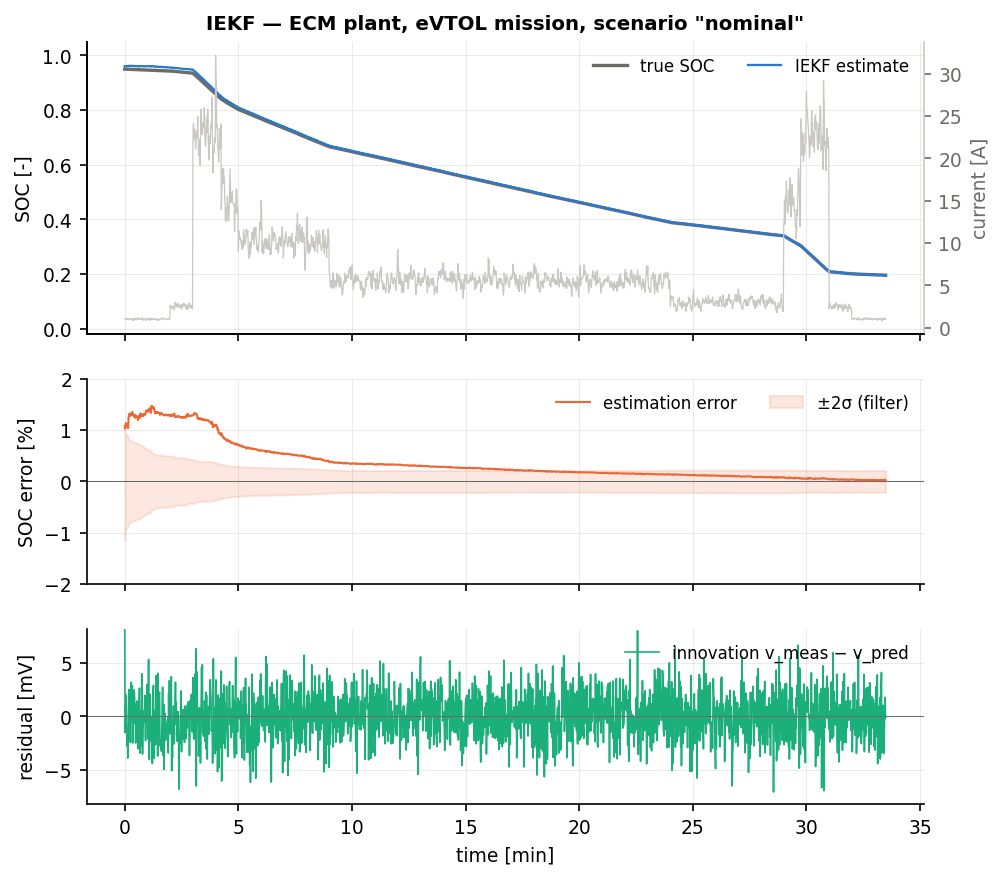
\includegraphics[width=\textwidth]{figures/cell_IEKF_nominal.png}
\caption{IEKF on the nominal eVTOL mission: true and estimated SOC (top), estimation error with the $\pm 2\sigma$ band when available (middle), voltage residual (bottom).}
\end{figure}
\begin{figure}[H]\centering
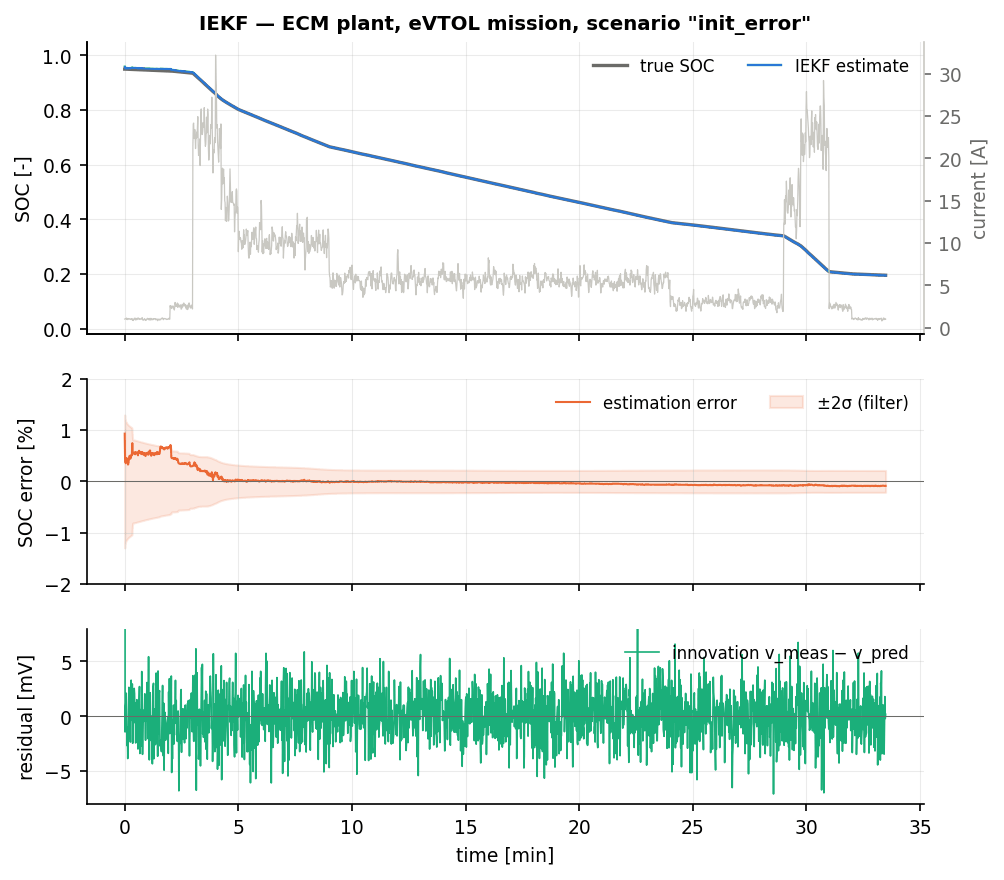
\includegraphics[width=\textwidth]{figures/cell_IEKF_init_error.png}
\caption{IEKF with a 35\,\% initial SOC error.}
\end{figure}

All numbers are three-seed means in per cent SOC.

On \texttt{nominal} the IEKF gives $\text{RMSE} = 0.30\,\%$, $\text{RMSE}_{\text{ss}} =
0.08\,\%$, against the EKF's $0.15/0.05\,\%$ --- slightly \emph{worse}. That is not a
contradiction: in nominal operation the innovations are at the millivolt level, the expansion
point barely moves, and the extra iterations only shuffle the correction between $\soc$ and the
RC and hysteresis states. The voltage-residual RMSE is identical to the EKF's
($0.79$\,mV for both), confirming that the two filters fit the measurement equally well and
differ only in how they distribute the correction.

Where a large innovation really occurs the iteration earns its keep. On \texttt{combined} the
EKF never converges ($12.44\,\%$) while the IEKF converges in the first sample and reaches
$2.13\,\%$ --- a factor of six better, obtained purely by relinearising, and the best maximum
error of the whole family on that scenario ($4.22\,\%$ against the EKF's $29.6\,\%$). On
\texttt{sensor\_dropout} ($15$\,s of stuck voltage) the IEKF gives $0.19\,\%$ against the EKF's
$0.46\,\%$ and the UKF's $0.86\,\%$, second only to the second-order EKF's $0.18\,\%$: after
the fault clears the
innovation is large and the first Gauss--Newton step is the wrong one, but the second and third
recover. \texttt{cold} improves slightly ($0.15\,\%$ against $0.16\,\%$) and \texttt{hot} is
unchanged at $0.03\,\%$.

The counter-example is \texttt{outliers} ($5\,\%$ of samples corrupted by $\pm 50$\,mV), where
the IEKF degrades to $0.36\,\%$ against the EKF's $0.21\,\%$ and the convergence metric is
pushed out to $242$\,s against $16$\,s. The reason is structural and worth stating plainly:
Gauss--Newton makes the filter fit the current measurement \emph{better}, and an outlier is a
measurement that must not be fitted at all. Iterating a least-squares update is the opposite of
robust estimation; when outliers are expected, the iteration must be combined with a robust
loss (Huber, Student-$t$) rather than used alone. \texttt{aged\_cell} ($1.69\,\%$ against
$1.52\,\%$) and \texttt{param\_mismatch} ($1.50\,\%$ against $1.36\,\%$) show a milder version
of the same effect: a better fit to a biased model is still biased.

Sensitivity to $J_{\max}$ was measured during development on four scenarios: $J = 1$ reproduces
the EKF exactly, $J = 2$ gives the best \texttt{combined} result, and $J = 3, 5, 10$ are
non-monotone. That non-monotonicity is a reminder that the iteration is solving the
\emph{wrong} problem slightly better: the MAP estimate of a model that is itself biased by an
unmodelled $25\,\%$ increase in $R_0$.

\paragraph{SPM plant: structured model error.}
\begin{figure}[H]\centering
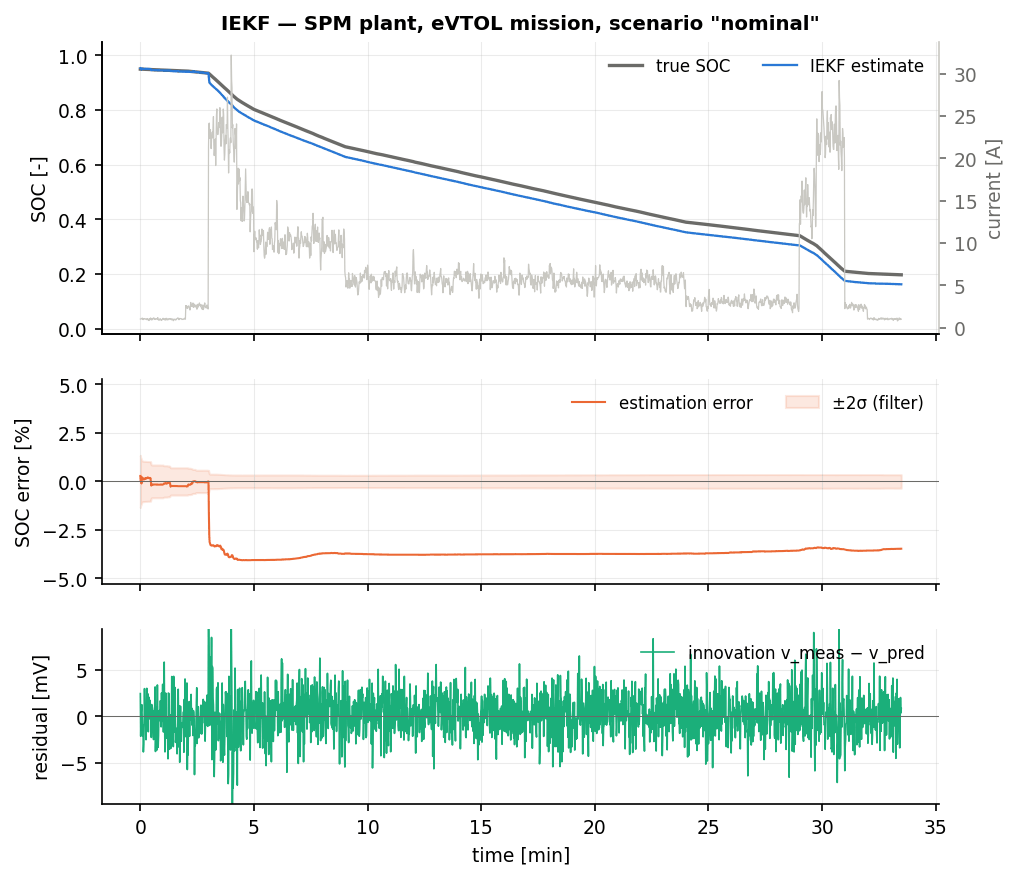
\includegraphics[width=\textwidth]{figures/cellspm_IEKF_nominal.png}
\caption{IEKF on the nominal mission with the electrochemical (SPM) plant.}
\end{figure}
The SPM block of the table is a different kind of test. The plant is the electrochemical
single-particle model; the estimator still runs a 2-RC equivalent circuit, fitted to that plant,
which leaves a \emph{structured} residual of about $4$\,mV (Butler--Volmer kinetics and
solid-phase diffusion that no 2-RC circuit can reproduce) and a slow second branch,
$\tau_2 = 556$\,s. Over a $33$-minute mission a $556$\,s pole barely relaxes, so $v_2(t)$ is
close to an affine ramp --- and so is $\ocv(\soc(t))$ while the cell discharges at a roughly
constant rate. The two channels through which the measurement sees the state,
$(\partial\ocv/\partial\soc)\,\delta\soc$ and $-\delta v_2$, are therefore nearly collinear in
the information accumulated over the flight: the pair $(\soc, v_2)$ is close to unobservable,
and no filter can decide whether a persistent few-millivolt residual belongs to the slow RC
branch or to the state of charge. Because that direction is weakly observable, a $4$\,mV
structured error maps onto \emph{several per cent} of SOC instead of the
$4\,\text{mV}/0.8\,\text{V}\approx0.5\,\%$ a well-conditioned channel would give. This
$(\soc,v_2)$ ambiguity, not the size of the residual, is the mechanism behind the
$3.7$--$4.6\,\%$ band in which the whole classical family sits.

The IEKF is marginally the best of the first-order Taylor-linearising filters here: $3.66\,\%$ on SPM
\texttt{nominal} against the EKF's $3.73\,\%$, $3.13\,\%$ on \texttt{init\_error} against
$3.81\,\%$, $2.87\,\%$ on \texttt{param\_mismatch} against $3.13\,\%$, $5.18\,\%$ on
\texttt{sensor\_dropout} against $5.31\,\%$. The improvements are real but small, and they are
of the same size as the improvement iterating buys on the ECM plant when the innovation is
large. What the iteration cannot do is resolve the ambiguity: relinearising more accurately at
the posterior does not add information along a direction in which the measurement carries
none, so the IEKF remains squarely inside the $3.7$--$4.6\,\%$ band. \texttt{cold} is in fact
slightly worse than the EKF's ($7.49\,\%$ against $7.35\,\%$), for the same reason
\texttt{outliers} was worse on the ECM plant: a tighter fit to a structurally wrong measurement
is not an improvement.

\section{Summary}
The IEKF costs one to four extra Jacobian evaluations per step
($0.56$--$0.60\,\SI{}{\micro\second}$ against the EKF's $0.44$--$0.48$) and converts the EKF's
one-shot linear update into a Gauss--Newton solve for the posterior mode. Use it when large
innovations are expected --- initialisation, post-fault recovery, sparse or infrequent
measurements --- and when the measurement function is strongly curved in the observed
direction; on this benchmark it turns the EKF's worst failure (\texttt{combined}, factor of
six) and its worst fault scenario (\texttt{sensor\_dropout}, factor of two) into good results.
Do not use it when the measurement stream contains outliers, because iterating fits them
harder, and do not expect it to fix over-confidence or structured model error: the covariance
is still first order and the SPM rows are within $2\,\%$ of the plain EKF's.
